\documentclass[tikz,border=8pt]{standalone}
% Shared look for every TikZ diagram. Load with \input{../../tools/tikz-style.tex}
\usepackage[T1]{fontenc}
\usepackage{lmodern}
\renewcommand{\sfdefault}{lmr}  % diagrams use the same serif as the text
\usetikzlibrary{arrows.meta, positioning, shapes.geometric, calc, fit, backgrounds}
\definecolor{cblue}{HTML}{4C78A8}
\definecolor{corange}{HTML}{F58518}
\definecolor{cgreen}{HTML}{54A24B}
\definecolor{cred}{HTML}{E45756}
\definecolor{cpurple}{HTML}{B279A2}
\definecolor{cgrey}{HTML}{6B6B6B}
\tikzset{
  every picture/.style={font=\sffamily, line width=1.2pt},
  box/.style={draw=#1, fill=#1!12, rounded corners=4pt, align=center, inner sep=7pt, minimum height=1.1cm},
  box/.default=cgrey,
  arrow/.style={-{Stealth[length=3mm]}, draw=cgrey, line width=1.4pt},
  title/.style={font=\sffamily\bfseries\Large},
  note/.style={font=\sffamily\small, text=cgrey, align=center},
}
\AtBeginDocument{\hyphenpenalty=10000 \exhyphenpenalty=10000}

\begin{document}
% Section 8: masked multi-head attention. Every head applies the causal mask inside its scaled dot-product
% attention, so every head's weight matrix is lower-triangular; the heads are concatenated and multiplied by W_O.
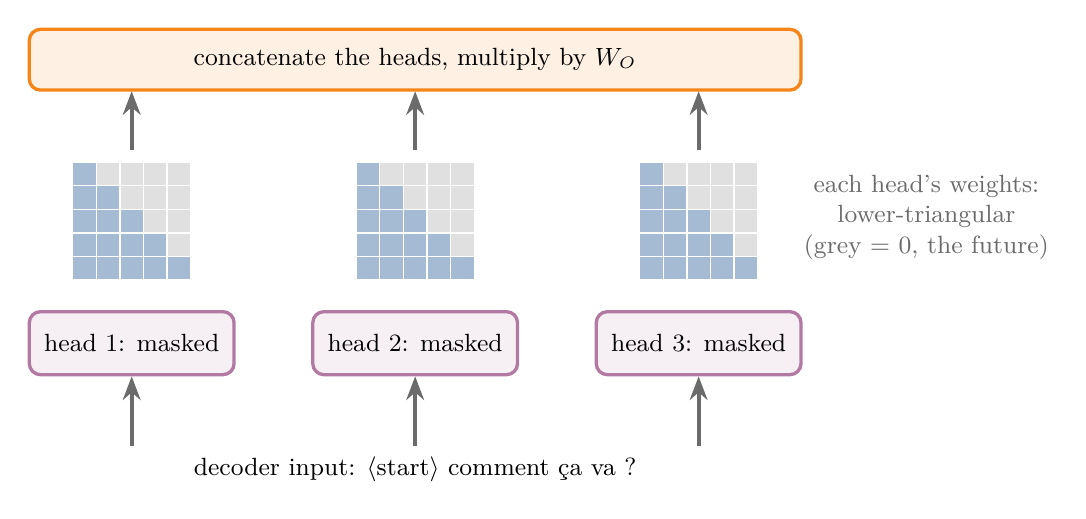
\begin{tikzpicture}[h/.style={box=cpurple, minimum width=2.6cm, minimum height=0.8cm, inner sep=3pt, font=\sffamily\small}]
  \foreach \k in {1,2,3} {
    \pgfmathsetmacro{\x}{3.6*\k - 3.6}
    \node[h] (h\k) at (\x, 0) {head \k: masked};
    \begin{scope}[shift={(\x - 0.75, 2.0)}, scale=0.3]
      \foreach \r in {0,...,4} \foreach \c in {0,...,4} {
        \pgfmathparse{\c > \r ? 1 : 0}
        \ifnum\pgfmathresult=1 \fill[black!12] (\c, -\r) rectangle ++(1, 1);
        \else \fill[cblue!50] (\c, -\r) rectangle ++(1, 1); \fi
        \draw[white, line width=0.5pt] (\c, -\r) rectangle ++(1, 1);
      }
    \end{scope}
    \draw[arrow] (\x, -1.3) -- (h\k.south);
    \draw[arrow] (\x, 2.45) -- (\x, 3.2);
  }
  \node[font=\sffamily\small] at (3.6, -1.6) {decoder input: $\langle$start$\rangle$ comment ça va ?};
  \node[box=corange, minimum width=9.8cm, minimum height=0.7cm, font=\sffamily\small] (cat) at (3.6, 3.6) {concatenate the heads, multiply by $W_O$};
  \node[note, anchor=west] at (8.4, 1.6) {each head's weights:\\lower-triangular\\(grey = 0, the future)};
\end{tikzpicture}
\end{document}
